\section{Q1:Visualization of quantization result of sample training / testing images}
\label{subsec:Q1_histograms}

\begin{figure}[htbp]
	\centering
	\begin{subfigure}[t]{0.3\linewidth}
		\centering
		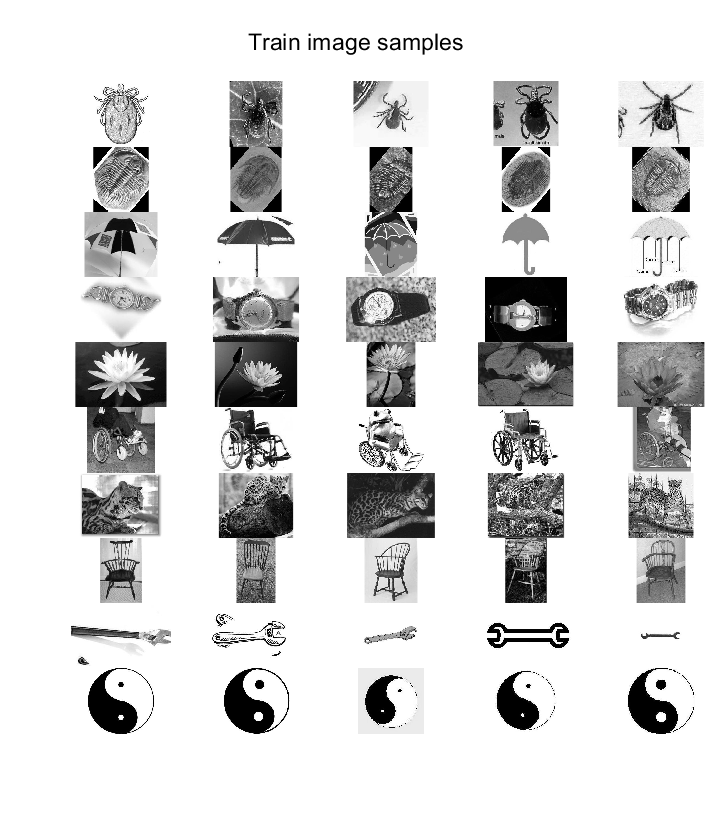
\includegraphics[height=6cm]{image/q1-appendix/train_img.png} 
		\caption{Train image samples}
	\end{subfigure}%
	\hfill
	\begin{subfigure}[t]{0.3\linewidth}
		\centering
		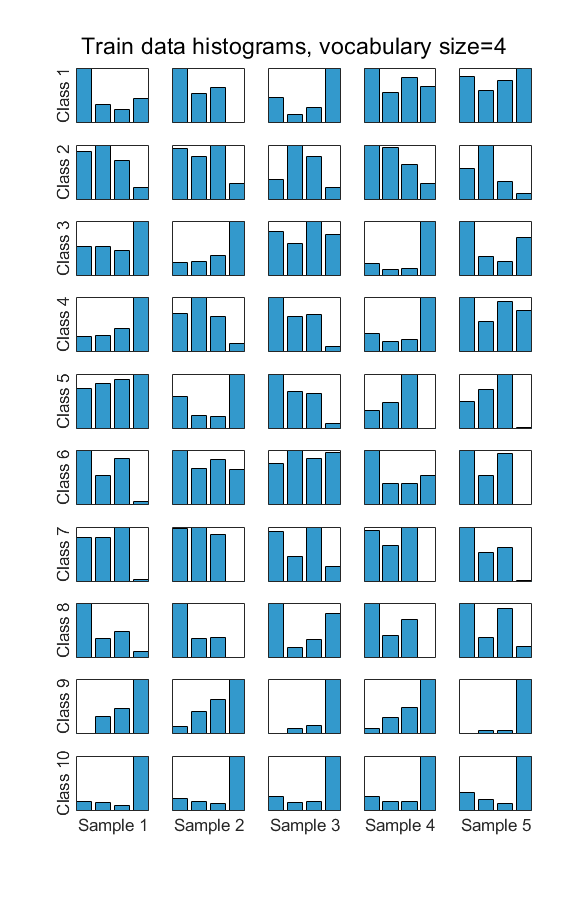
\includegraphics[height=6cm]{image/q1-appendix/train_4.png}
		\caption{Train data quantisation result, $K=4$}
	\end{subfigure}
	\hfill
	\begin{subfigure}[t]{0.3\linewidth}
		\centering
		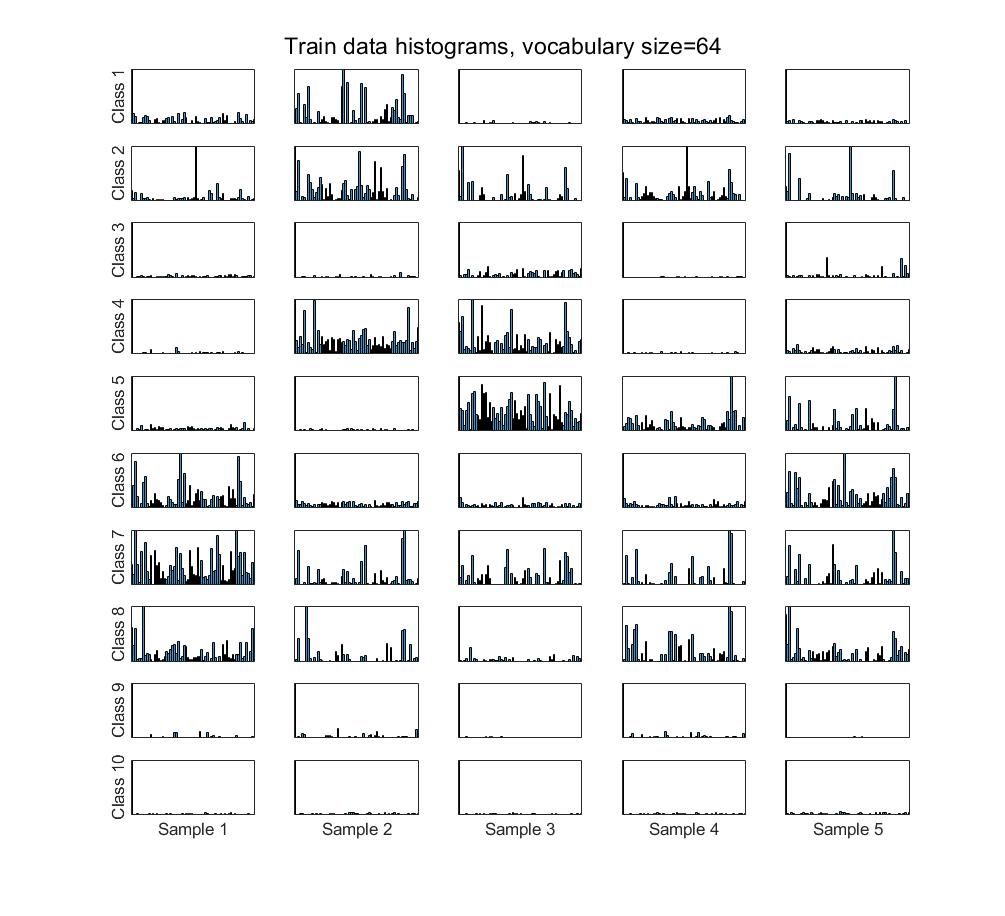
\includegraphics[height=6cm]{image/q1-appendix/train_64.png}
		\caption{Train data quantisation result, $K=64$}
	\end{subfigure}
	\caption{Visualistaion of train data quantisation result}
	\label{fig:q1_histogram_tr}
\end{figure}

\begin{figure}[htbp]
	\centering
	\begin{subfigure}[t]{0.3\linewidth}
		\centering
		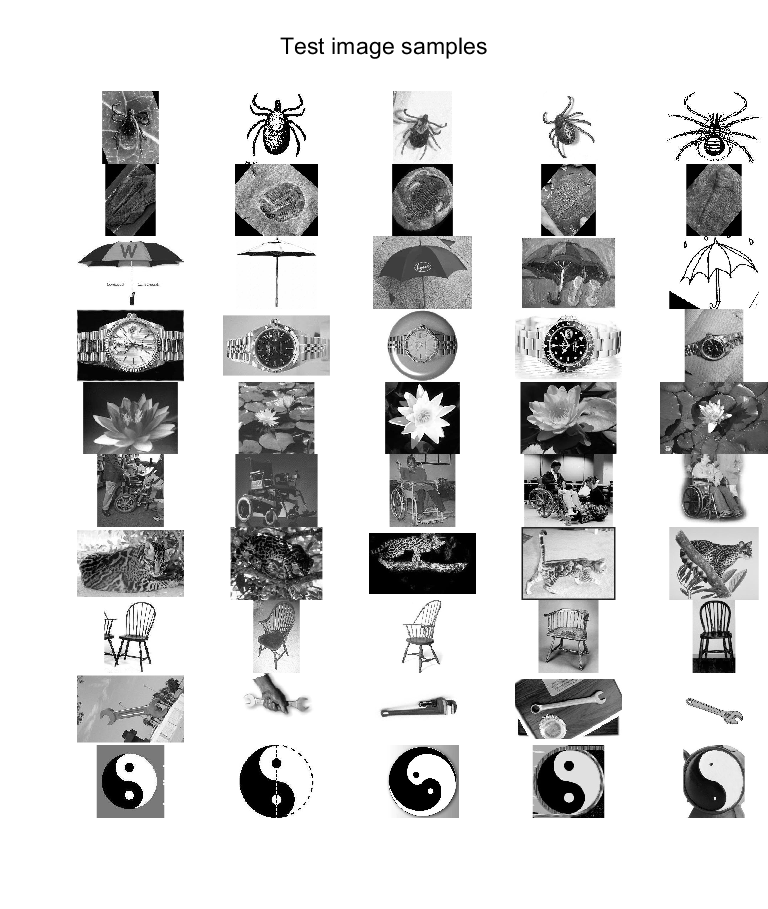
\includegraphics[height=6cm]{image/q1-appendix/test_img.png} 
		\caption{Test image samples}
	\end{subfigure}%
	\hfill
	\begin{subfigure}[t]{0.3\linewidth}
		\centering
		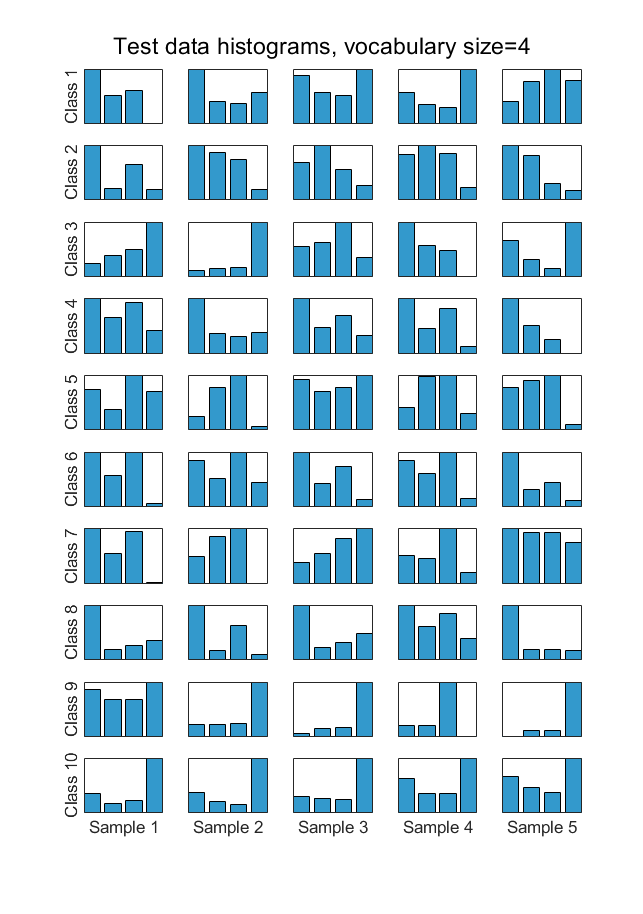
\includegraphics[height=6cm]{image/q1-appendix/test_4.png}
		\caption{Test data quantisation result, $K=4$}
	\end{subfigure}
	\hfill
	\begin{subfigure}[t]{0.3\linewidth}
		\centering
		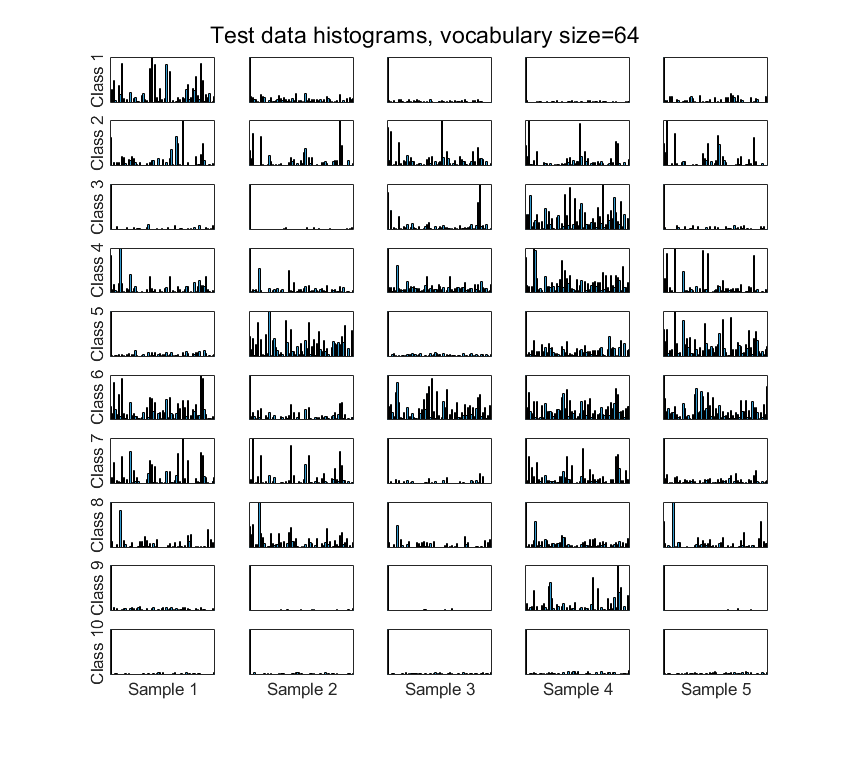
\includegraphics[height=6cm]{image/q1-appendix/test_64.png}
		\caption{Test data quantisation result, $K=64$}
	\end{subfigure}
	\caption{Visualistaion of test data quantisation result}
	\label{fig:q1_histogram_te}
\end{figure}

\section{Q1:Cosine similarity between images in \cref{fig:q1-fig2}}
\label{subsec:Q1_cossim}
\begin{figure}[htbp]
	\centering
	\begin{subfigure}[t]{0.25\linewidth}
		\centering
		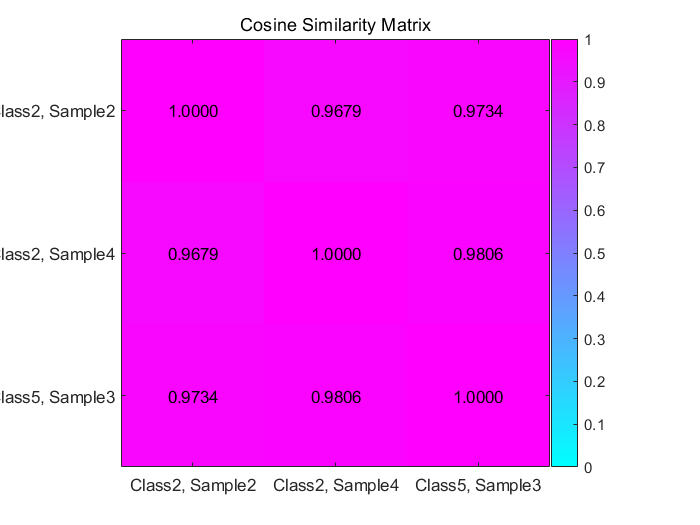
\includegraphics[width=\linewidth]{image/q1-appendix/similarity_4.png} 
		\caption{$K=4$}
	\end{subfigure}%
	\hfill
	\begin{subfigure}[t]{0.25\linewidth}
		\centering
		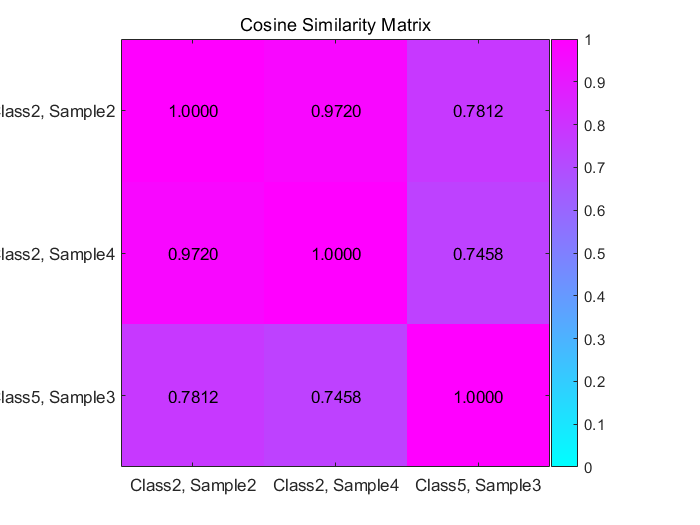
\includegraphics[width=\linewidth]{image/q1-appendix/similarity_16.png} 
		\caption{$K=16$}
	\end{subfigure}%
	\hfill
	\begin{subfigure}[t]{0.25\linewidth}
		\centering
		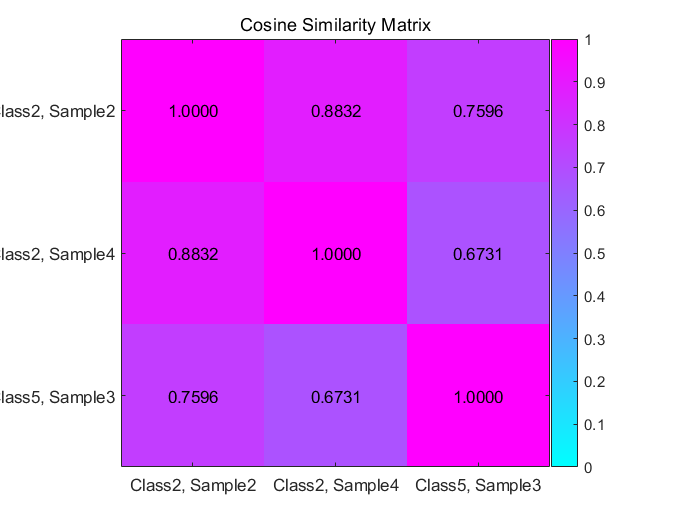
\includegraphics[width=\linewidth]{image/q1-appendix/similarity_64.png} 
		\caption{$K=64$}
	\end{subfigure}%
	\hfill
	\begin{subfigure}[t]{0.25\linewidth}
		\centering
		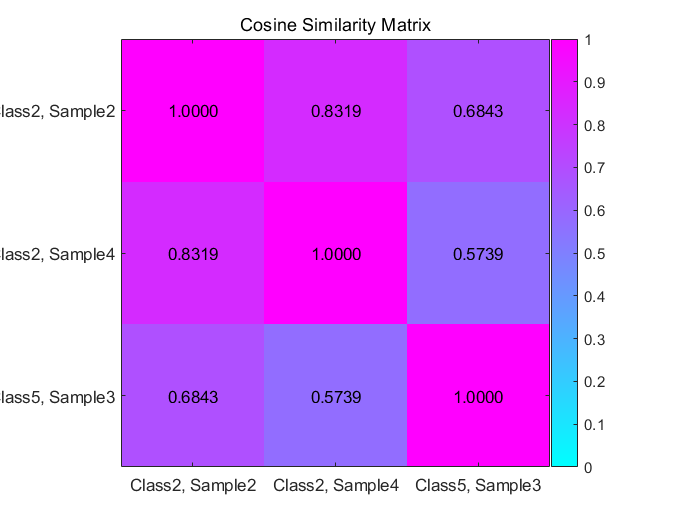
\includegraphics[width=\linewidth]{image/q1-appendix/similarity_256.png} 
		\caption{$K=256$}
	\end{subfigure}%
	\caption{Visualization of cosine similarity matrix of \cref{fig:q1-fig2} according to the different $K$}
	\label{fig:q1_cossim}
\end{figure}

\section{Q2: Test result's confusion matrix and success/failure cases}
\label{subsec:Q2-app1}

\section{Q2: Visualization of random forest's information gain process}
\label{subsec:Q2-app2}


\section{Q3: Optimization process of Random forest vocabulary}
\label{subsec:Q2-app3}
\begin{figure}[htbp]
	\centering
	\begin{subfigure}[H]{0.7\linewidth}
		\centering
		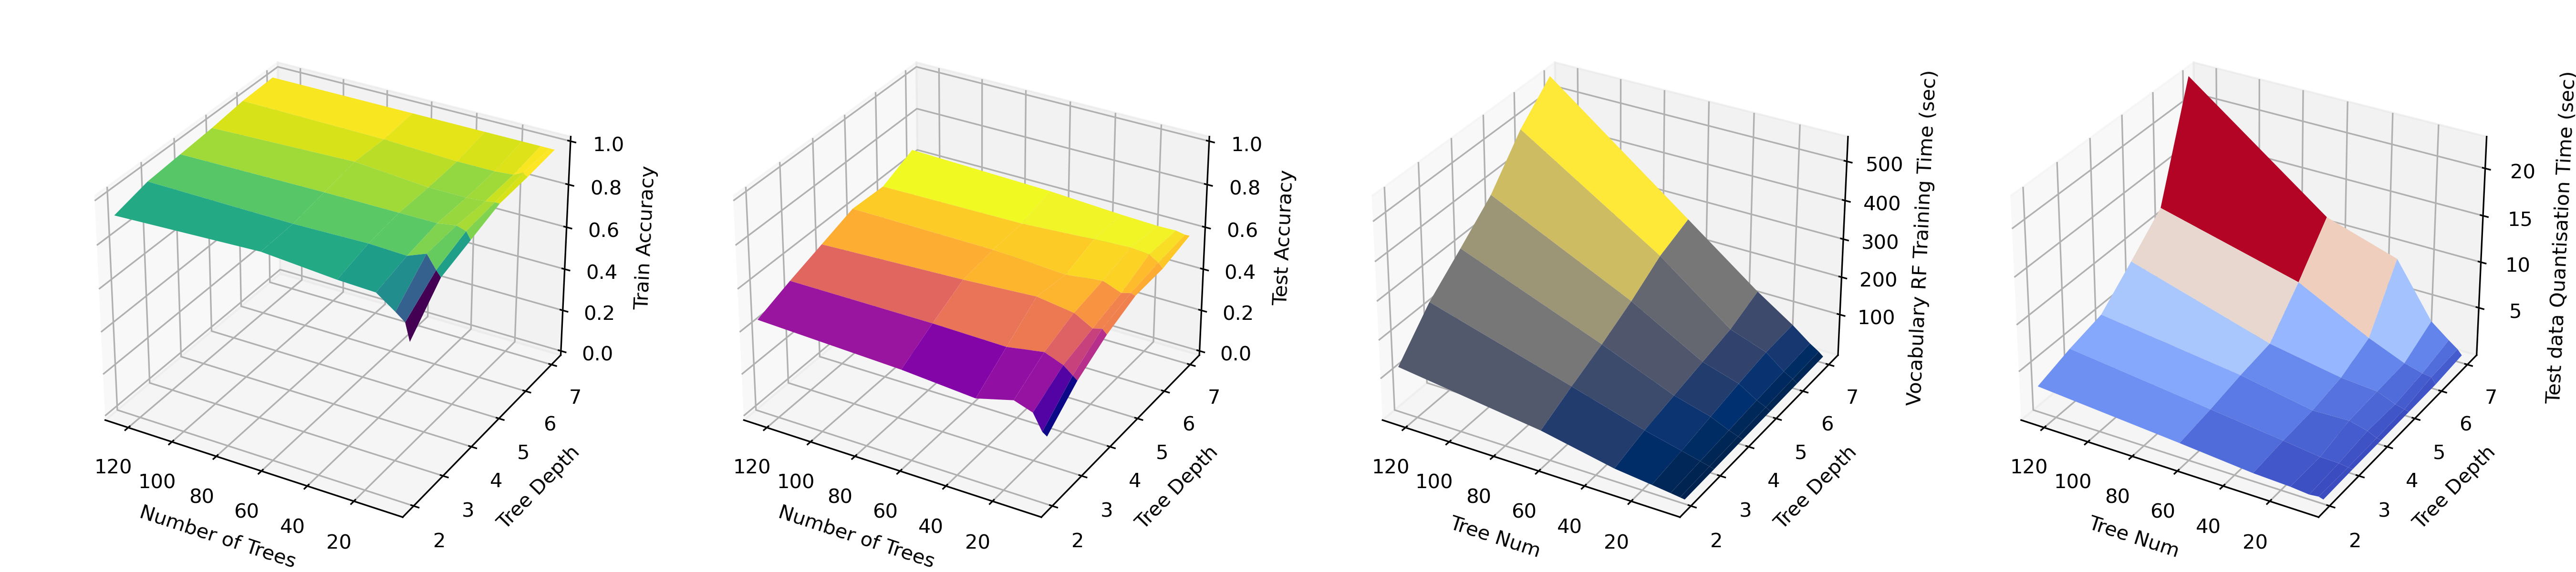
\includegraphics[width=\linewidth]{image/q3-fig1.png}
		\caption{Training\&Testing accuracy and time according to the number of tree and the depth of tree}
		\label{fig:q3-fig1}
	\end{subfigure}
	\begin{subfigure}[H]{0.7\linewidth}
		\centering
		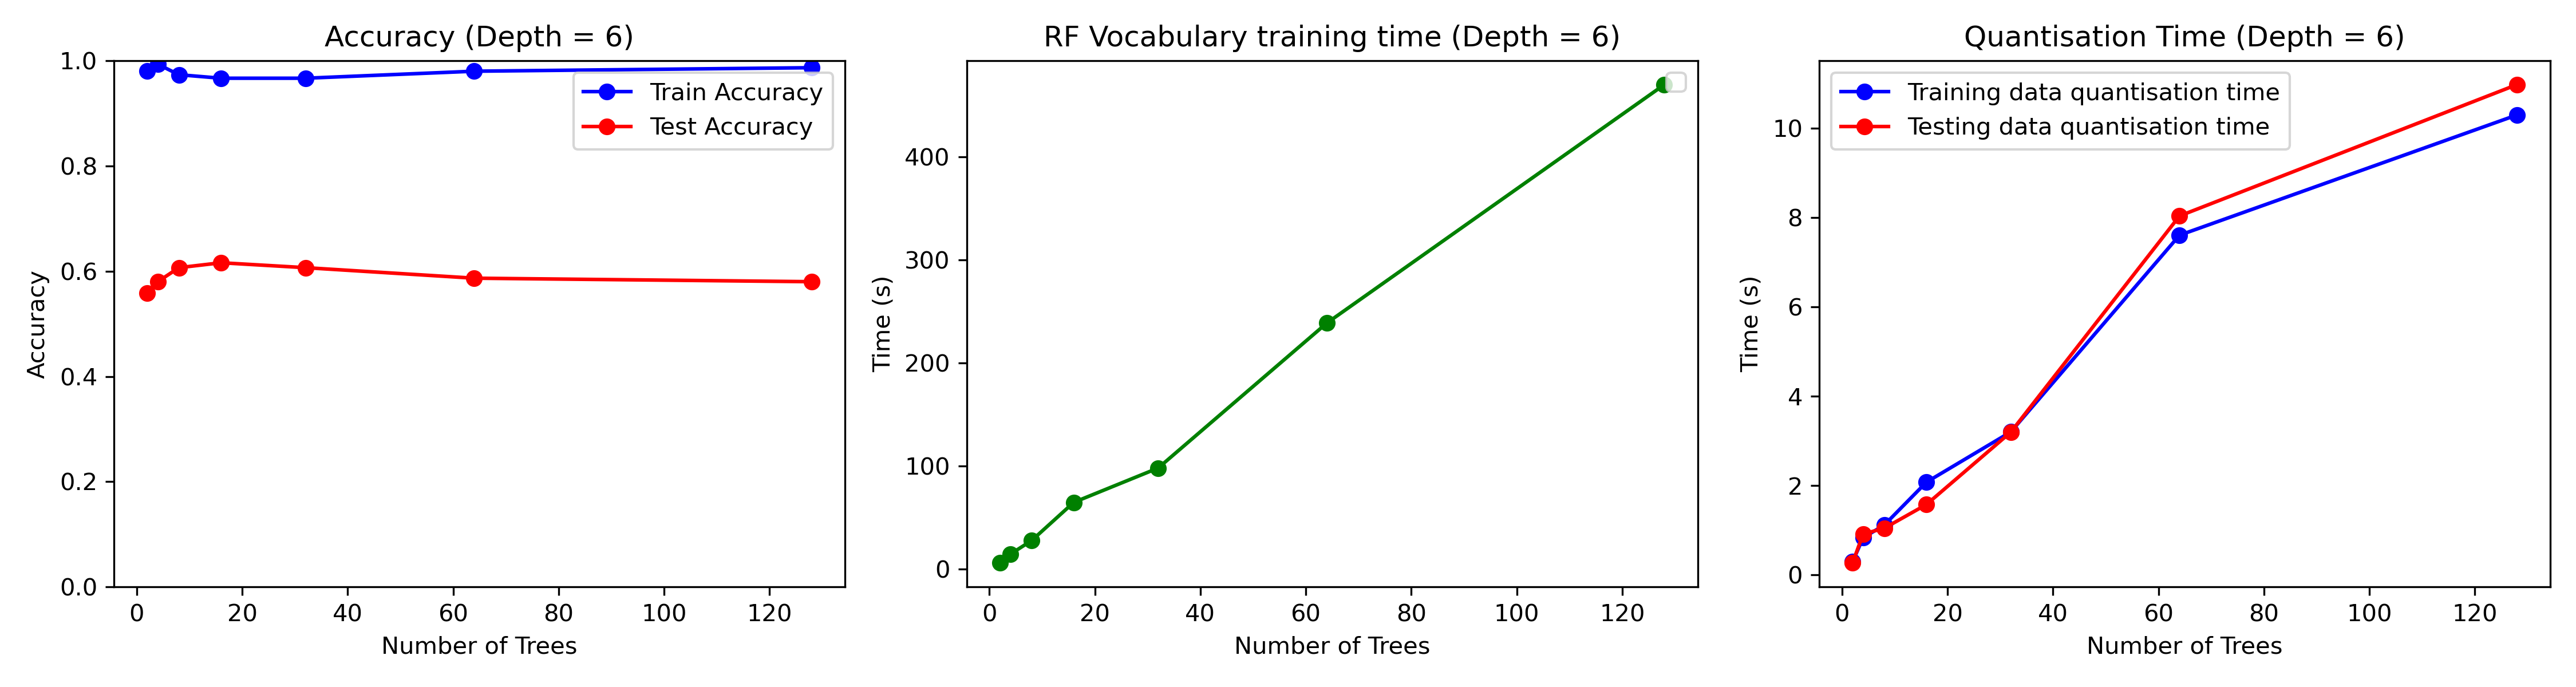
\includegraphics[width=\linewidth]{image/q3-fig2.png}
		\caption{Training\&Testing accuracy and time according to the number of tree (D = 8)}
		\label{fig:q3-fig2}
	\end{subfigure}
	\begin{subfigure}[H]{0.7\linewidth}
		\centering
		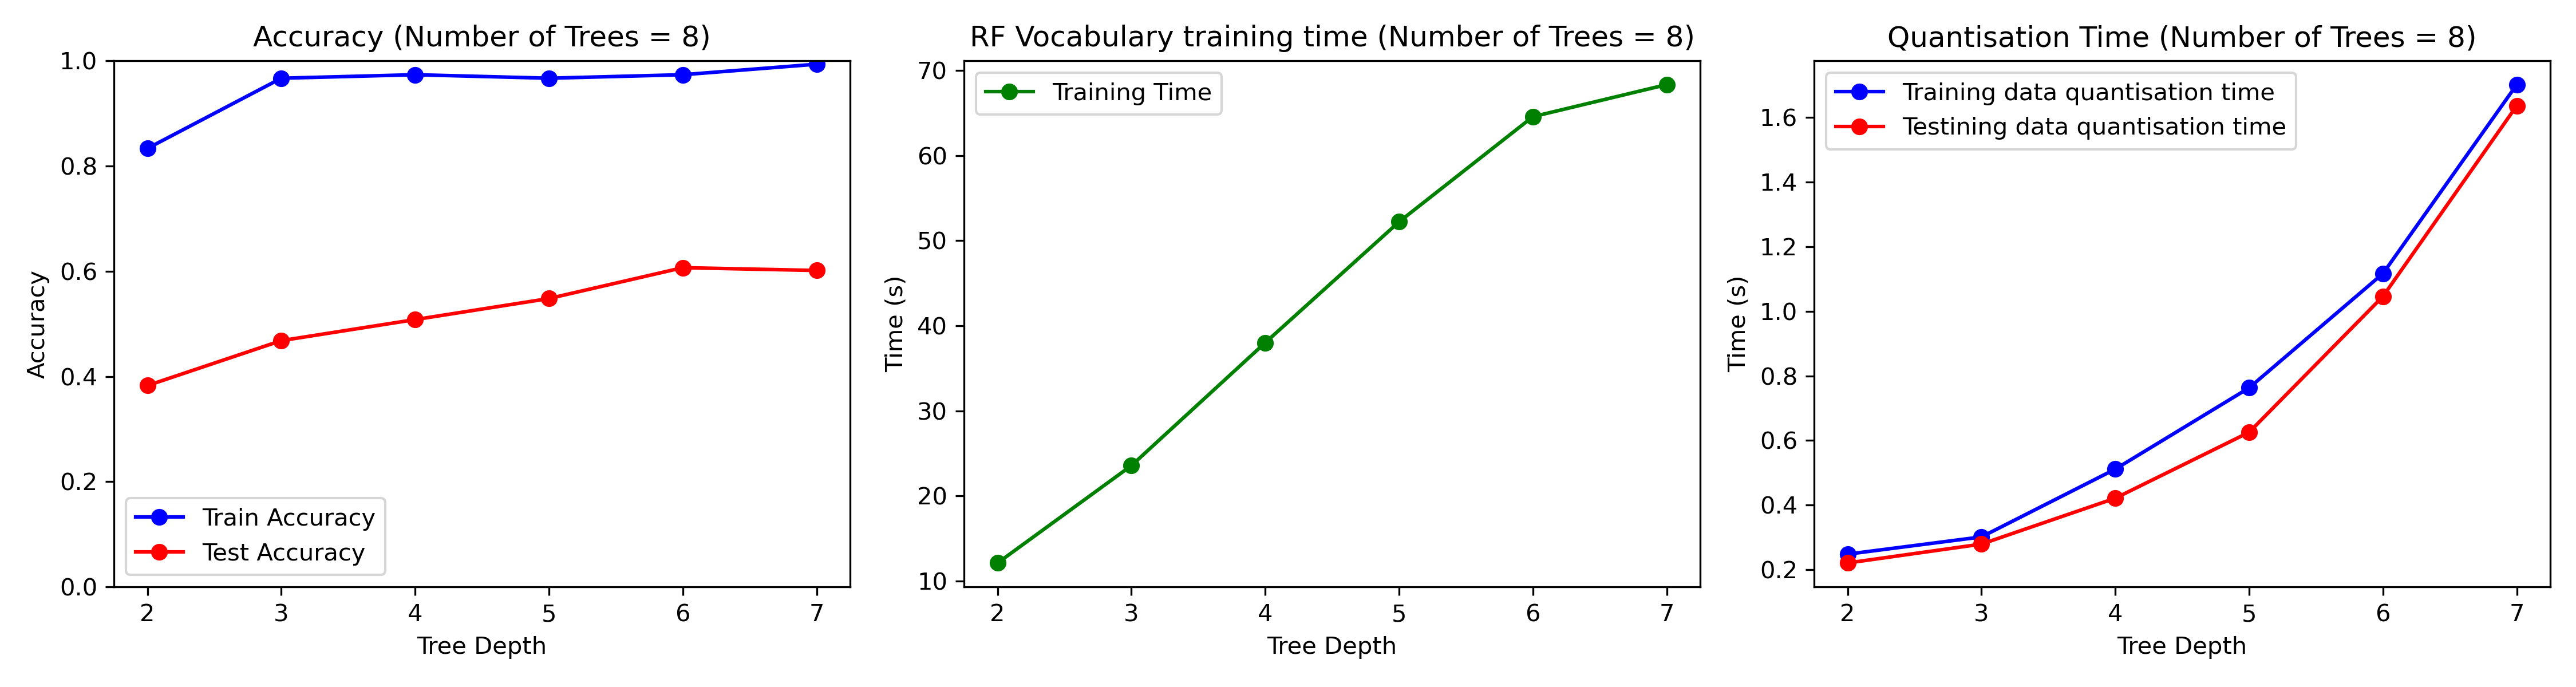
\includegraphics[width=\linewidth]{image/q3-fig3.png}
		\caption{Training\&Testing accuracy and time according to the depth of tree (N = 250)}
		\label{fig:q3-fig3}
	\end{subfigure}
	\caption{Training\&Testing accuracy and time according to the number and depth of trees}
\end{figure}


\begin{figure}[htbp]
	\centering
	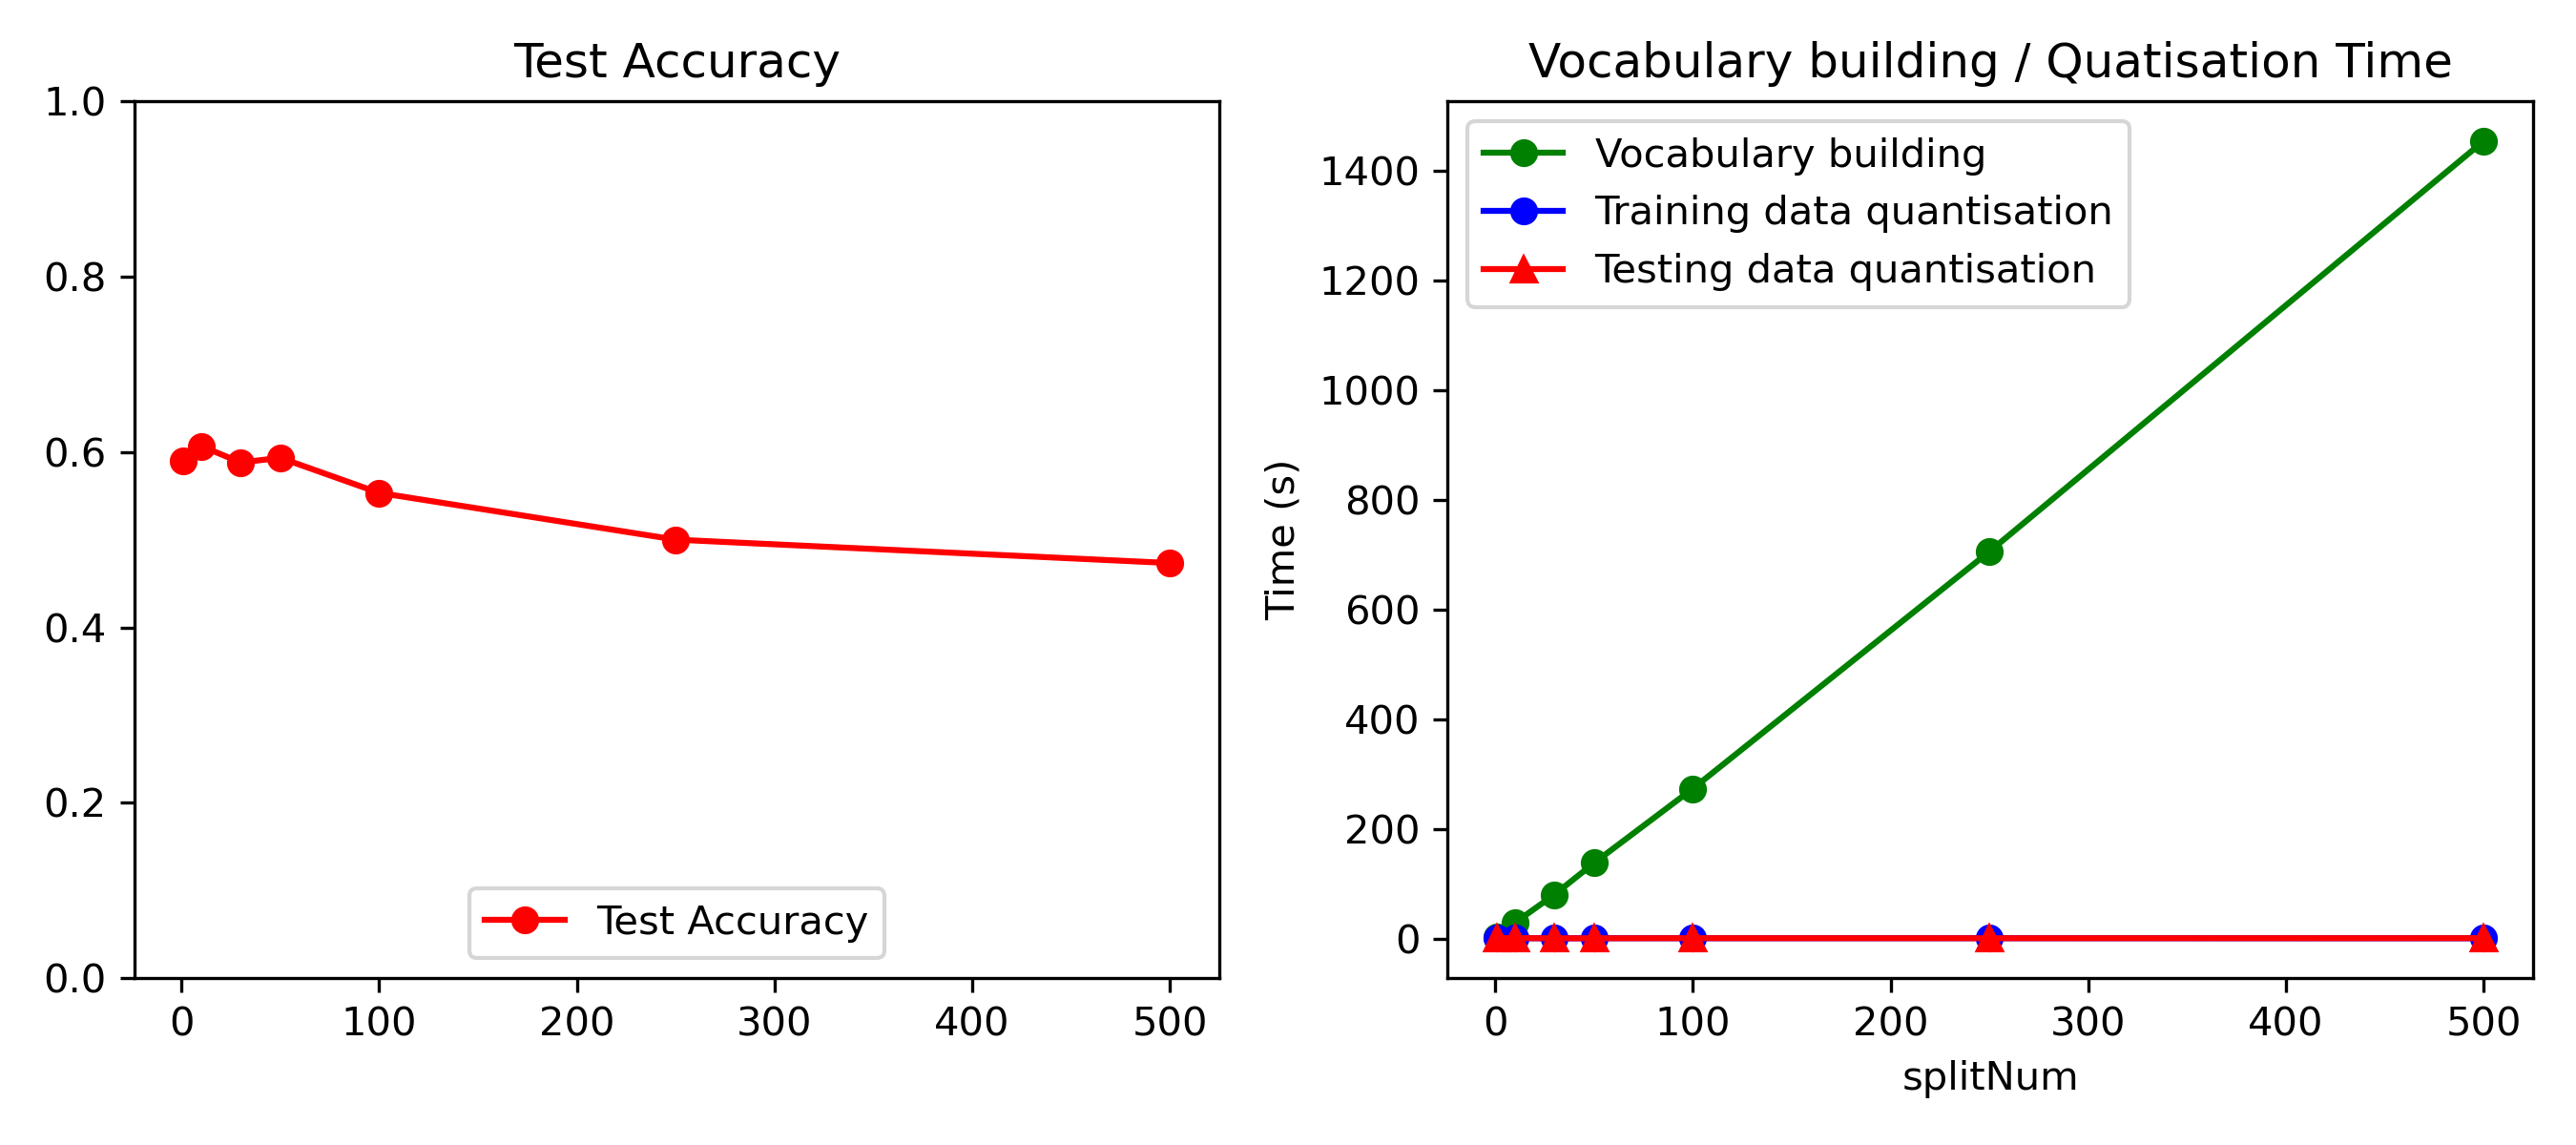
\includegraphics[width=0.5\linewidth]{image/q3-fig5.png}
	\caption{Training\&Testing accuracy and time according to the randomness parameter}
	\label{fig:q3-fig5}
\end{figure}

\section{Q3: K-means and Random forest vocabularies' theoretical properties}
\label{subsec:Q3-app1}
\begin{table}[htbp]
	\centering
	\setlength{\tabcolsep}{6pt} % Adjust column spacing
	\renewcommand{\arraystretch}{1.5} % Adjust row height
	\resizebox{0.5\textwidth}{!}{ % Scale table to fit text width
		\begin{tabular}{|c||c|c|}
			\hline
			& K-means & Random forest \\ \hline\hline
			Training time & 99.50 & $O(ND\rho \times \text{(number of training data)})$ \\ \hline
			Testing time & 97.80 & $O(ND \times \text{(number of testing data)})$ \\ \hline
			Space complexity & 100.00 & $O(2^{D} \times N)$ \\ \hline
		\end{tabular}
	}
	\caption{Theoretical properties of vocabulary method: K-means and RF}
	\label{table:q3-app-1}
\end{table}

\section{Q3: Difference between K-means and RF vocabularies' quantisation result}
\label{subsec:Q3-app2}

